\documentclass[10pt,aspectratio=149]{beamer}

\usecolortheme{Calm}
\usetheme{Calm}

%%\usepackage{minted}
%%\usemintedstyle{pastie}

\usepackage{pgfplots}
\usepackage{pgfplotstable}
\usepackage[utf8]{inputenc}
\usetikzlibrary{shapes, arrows, positioning}

\author{Steve Vissault, Matthew Talluto, \\
Isabelle Boulangeat and Dominique Gravel}
\title{Difficult migration of temperate tree species \\
in the boreal forest under climate change?}
\date{\today}
\institute{Université du Québec à Rimouski}

\begin{document}
\begin{frame}[plain]
   \titlepage
\end{frame}

%%% Keys
%1. Le titre
%2. Travail collaboratif qui regroupe plusieurs chercheurs du laboratoire d'écologie théorique de dominiaue gravel
%3. Fruit de 1 ans de travail dans le cadre de ma maitrise
%4. Cette présentation a pour objectif de montrer quelques résultats préliminaires


%%%%%%%%%%%%%%%%%%%%%%%%%%%%%%%%%%%%%%%%%%%%%%%%%%%%%%%%%%%%%%%%%%%%%%%%%%%%%%%%%%%%%%%%%%%%%%%%
%%% Objective

%%% 1. L'un des objectifs de ce mémoire consiste à évaluer les changements dans l'aire de répartition de la communauté de la forêt nordique du Québec ainsi que son taux de migration sous l'effet des changements climatiques 

%%% 2. Lorsque l'on parle de migration et de changement d'aire de répartition d'une espèce dans ce cas-ci d'une communauté, on s'intéresse particulièrement à la distance et au de migration. 

\begin{frame}{Introduction}{Objective}

\textbf{Main objective:} Assess range shift and migration rate of the temperate forest community toward boreal forest under climate change.

\pause 

\vspace{1em}
\textbf{Why ?}
		\begin{itemize}
			\item Predict the future distribution of temperate species community in Quebec
		 	\item Improve and adapt our forests management practices under CC
		\end{itemize}

\end{frame}

%%%%%%%%%%%%%%%%%%%%%%%%%%%%%%%%%%%%%%%%%%%%%%%%%%%%%%%%%%%%%%%%%%%%%%%%%%%%%%%%%%%%%%%%%%%%%%%%
%%% Context

\begin{frame}{Context}{The boreal-temperate ecotone}

The surface of the boreal-temperate forests ecotone is \textbf{expected to shift in the next decades}.

\begin{figure}
	\includegraphics[width=.70\paperwidth]{Figs/ecotone.pdf}
\end{figure}

   \paper{Goldblum and Rig, 2010}
\end{frame}

%% 


%%%%%%%%%%%%%%%%%%%%%%%%%%%%%%%%%%%%%%%%%%%%%%%%%%%%%%%%%%%%%%%%%%%%%%%%%%%%%%%%%%%%%%%%%%%%%%%%
%%% Context

\begin{frame}{Context}{The boreal-temperate ecotone}

1. The location of this ecotone is \textbf{responsive to the climate}.

\begin{figure}
	\includegraphics[width=.70\paperwidth]{Figs/climecotone.png}
\end{figure}

   \paper{Goldblum and Rig, 2010}
\end{frame}

%%%%%%%%%%%%%%%%%%%%%%%%%%%%%%%%%%%%%%%%%%%%%%%%%%%%%%%%%%%%%%%%%%%%%%%%%%%%%%%%%%%%%%%%%%%%%%%%
%%% SDM

\begin{frame}{Context}{Future species distribution predicted}

2. Several temperate forest species are predicted to \textbf{shift northward} under CC
\begin{columns}[c]
	\begin{column}{.40\paperwidth}
	\textbf{For instance:}
		\begin{itemize}
			\item Sugar maple
			\item Yellow birch
			\item American ash
			\item Red oak
			\item ...
		\end{itemize}
		%Fewer species show a direction of migration (predicted) consistant with data observed (Zhu \textit{et al}, 2012)
	\end{column}
	\begin{column}{.40\paperwidth}
	\pause
		\begin{figure}
			\includegraphics[width=.38\paperwidth]{Figs/sugar_map_distrib.jpg}
		\end{figure}
	\scriptsize{\textbf{Future climate enveloppe of Sugar maple (2071-2100)} - McKenney \textit{et al}, 2007}
	\end{column}
\end{columns}
   \paper{McKenney \textit{et al}, 2007; Woodall \textit{et al}, 2008; Iverson and Prasad, 2002}
\end{frame}

%%% SDM are limited in this study context
% Centered on species
% Abiotic conditions (e.g. Climate, soil)
% Spatially implicit
% Instantaneous dynamic
			  

%%%%%%%%%%%%%%%%%%%%%%%%%%%%%%%%%%%%%%%%%%%%%%%%%%%%%%%%%%%%%%%%%%%%%%%%%%%%%%%%%%%%%%%%%%%%%%%%
%%% Tools

%%% Quand on s'intéresse au changements d'aire de répartition d'un communauté, deux processus sont à prendre en considérations:
\begin{frame}{New approach}{Which tool is more appropriate?}

\textbf{Forest have:}
		\begin{enumerate}
			\item Limited dispersions
			\item Slow population dynamics
			\item Successional stages based on facilitation and/or competition processes
		\end{enumerate}
\vspace{1em}
\pause
\textbf{To predict species range shift, we need to include \alert{two processes:}}
	\begin{itemize}
		\item Distance of colonization %(Seeds dispersion ability): Size of the patch, ecological knowledges
		\item Dispersal rate %(immigration and establishment phases). 
		% Ces deux processus vont être altérer sous l'effet des CC
	\end{itemize}
	\pause
	\alert{Those processes are affected by the future climate}

\end{frame}

%%%%%%%%%%%%%%%%%%%%%%%%%%%%%%%%%%%%%%%%%%%%%%%%%%%%%%%%%%%%%%%%%%%%%%%%%%%%%%%%%%%%%%%%%%%%%%%%
%%% Tools

\begin{frame}{New approach}{Which tool is more appropriate?}
	
\textbf{Diagram: Model tools}	
	
\end{frame}

%%%%%%%%%%%%%%%%%%%%%%%%%%%%%%%%%%%%%%%%%%%%%%%%%%%%%%%%%%%%%%%%%%%%%%%%%%%%%%%%%%%%%%%%%%%%%%%%
%% Generality of the model 

\begin{frame}{Method}{State and Transitional Model}

\begin{columns}[c]
	\begin{column}[c]{.40\paperwidth}
		\begin{figure}
			\small{\input{Figs/fig_wo_params.tikz}}
		\end{figure}
	\end{column}
	\begin{column}[l]{.50\paperwidth}
		\begin{itemize}
			\item Lanscape modelling scale
			\item 4 States (\textbf{R},\textbf{B},\textbf{T},\textbf{M})
			\item \textbf{R} corresponds to a post-disturbance patch
			\item Probability of transition given climatic conditions
			\item Spatially explicit and stochastic model
		\end{itemize}
	\end{column}
\end{columns}
\end{frame}

%%%%%%%%%%%%%%%%%%%%%%%%%%%%%%%%%%%%%%%%%%%%%%%%%%%%%%%%%%%%%%%%%%%%%%%%%%%%%%%%%%%%%%%%%%%%%%%%
%% Generality of the model 

\begin{frame}{Method}{State and Transitional Model}

\begin{columns}[c]
	\begin{column}[c]{.40\paperwidth}
		\begin{figure}
			\small{\input{Figs/fig_wo_params.tikz}}
		\end{figure}
	\end{column}
	\begin{column}[l]{.50\paperwidth}
	\begin{table}
		\begin{tabular}{|l|l|}
			\hline
			\textbf{States}  & \textbf{Classification}\\
			\hline
			T & $Ba_t \geq 75\%$    \\
			M & $Ba_b \geq 25\%$ and $Ba_t \geq 25\%$ \\
			B & $Ba_b \geq 75\%$   \\
			R & $Ba_r  \geq 75\%$ \\
			\hline
		\end{tabular}
		\end{table}
		\textbf{See with Dom for the new classification}
	\end{column}
\end{columns}

\end{frame}

%%%%%%%%%%%%%%%%%%%%%%%%%%%%%%%%%%%%%%%%%%%%%%%%%%%%%%%%%%%%%%%%%%%%%%%%%%%%%%%%%%%%%%%%%%%%%%%%
%% Paremeters description 

\begin{frame}{Method}{State and Transitional Model}

\begin{columns}[c]
	\begin{column}[c]{.40\paperwidth}
		\begin{figure}
			\small{\begin{center}

\tikzstyle{noeud}=[circle,
	thick,
	minimum size = 1cm,
	inner sep =5pt,
	draw=QUICCgreen,
	fill=QUICCgreen]

\begin{tikzpicture}[->,>=stealth',auto,scale=0.45]
	\node [circle,noeud] (M) at (0,0) {\color{white}\textbf{M}};
	\node [circle,noeud] (B) at (-5,5) {\color{white}\textbf{B}};
	\node [circle,noeud] (T) at (5,5) {\color{white}\textbf{T}};
	\node [circle,noeud] (R) at (0,10) {\color{white}\textbf{R}};

	\draw[thick,-latex] (M) to[bend right=10] node[above,sloped] {\footnotesize Exclusion} (B);
	\draw[thick,-latex] (B) to[bend right=10] node[below,sloped] {\footnotesize Colonization} (M);

	\draw[thick,-latex] (T) to[bend right=10] node[above,sloped] {\footnotesize Colonization} (M);
	\draw[thick,-latex] (M) to[bend right=10] node[below,sloped] {\footnotesize Exclusion} (T);

	\draw[thick,-latex] (T) to[bend right=10] node[above,sloped] {\footnotesize Disturbance} (R);
	\draw[thick,-latex] (R) to[bend right=10] node[below,sloped] {\footnotesize Succession} (T);

	\draw[thick,-latex] (R) to[bend right=10] node[above,sloped] {\footnotesize Succession} (B);
	\draw[thick,-latex] (B) to[bend right=10] node[below,sloped] {\footnotesize Disturbance} (R);

	\draw[thick,-latex,transform canvas={xshift=0.6ex}] (R) to node[above,sloped] {\footnotesize Succession} (M);
	\draw[thick,-latex,transform canvas={xshift=-0.6ex}] (M) to node[above,sloped] {\footnotesize Disturbance} (R);
\end{tikzpicture}
\end{center}

}
		\end{figure}
	\end{column}
	\begin{column}[l]{.50\paperwidth}
	\textbf{Parameters}:
	\begin{itemize}
		\item $\beta$: Colonization rate
		\item $\theta$: Succession rate
		\item $\phi$: Regeneration functions
		\item $\epsilon$: Disturbance rate
	\end{itemize}
	\vspace{1em}
	\textbf{Each rate depends of}:
		\begin{itemize}
			\item Proportion of states available in the neighborhood
			\item Climatic conditions encounter by the patch (Precipitation, Temperature)
		\end{itemize}
	\end{column}
\end{columns}

\end{frame}


%%%%%%%%%%%%%%%%%%%%%%%%%%%%%%%%%%%%%%%%%%%%%%%%%%%%%%%%%%%%%%%%%%%%%%%%%%%%%%%%%%%%%%%%%%%%%%%%
%%% Data

\begin{frame}{Data used}{The quicc-for database}
	\center Merge several databases of forest permanent plots survey
\begin{figure}
	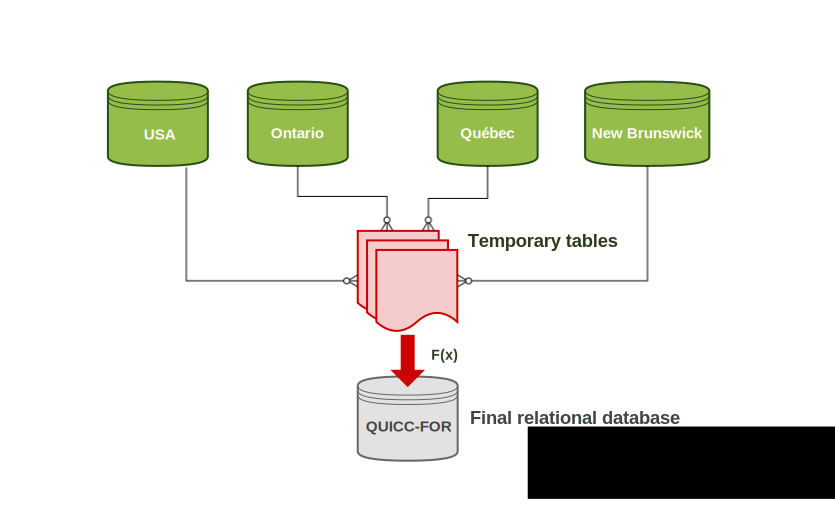
\includegraphics[width=.60\paperwidth]{Figs/quiccfor.pdf}
\end{figure}

\end{frame}

%%%%%%%%%%%%%%%%%%%%%%%%%%%%%%%%%%%%%%%%%%%%%%%%%%%%%%%%%%%%%%%%%%%%%%%%%%%%%%%%%%%%%%%%%%%%%%%%
%%% Data

\begin{frame}[t]{Data used}{Calibration}
	\center Preliminary results include only the Quebec database
\begin{figure}
	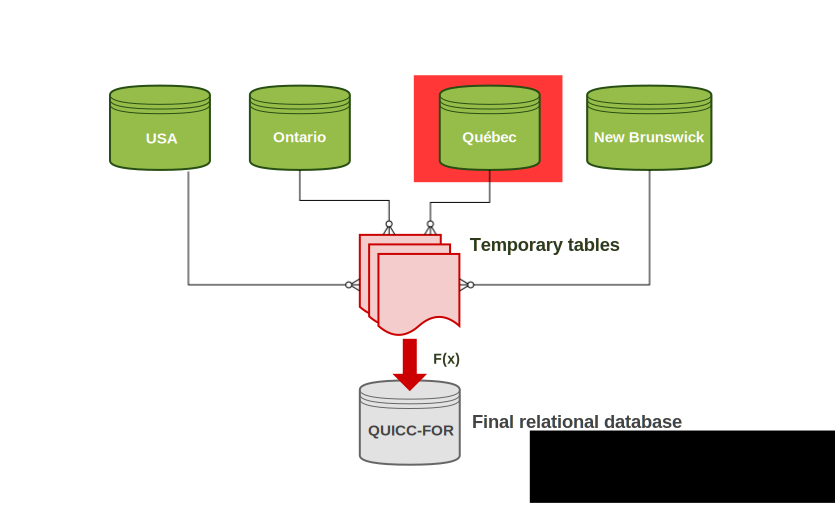
\includegraphics[width=.60\paperwidth]{Figs/quiccfor2.pdf}
\end{figure}

\end{frame}


%%%%%%%%%%%%%%%%%%%%%%%%%%%%%%%%%%%%%%%%%%%%%%%%%%%%%%%%%%%%%%%%%%%%%%%%%%%%%%%%%%%%%%%%%%%%%%%%
%%% Data

\begin{frame}[t]{Data used}{Calibration}
	
	\textbf{Maps and desc plots included}

\end{frame}

%%%%%%%%%%%%%%%%%%%%%%%%%%%%%%%%%%%%%%%%%%%%%%%%%%%%%%%%%%%%%%%%%%%%%%%%%%%%%%%%%%%%%%%%%%%%%%%%
%% Explicit version 

\begin{frame}{Method}{State and transitional model spatially explicit}

\begin{columns}[c]
	\begin{column}[c]{.40\paperwidth}

	\textbf{Raster informations}

	\end{column}
	\begin{column}[c]{.40\paperwidth}
		
	\textbf{Probability space}

	\end{column}
\end{columns}

\end{frame}


%%%%%%%%%%%%%%%%%%%%%%%%%%%%%%%%%%%%%%%%%%%%%%%%%%%%%%%%%%%%%%%%%%%%%%%%%%%%%%%%%%%%%%%%%%%%%%%%
%%% Resultats

\begin{frame}{Results}{Probabilities distribution}

\begin{centering}
	\textbf{Figure: PDFs}
\end{centering}

\end{frame}


%%%%%%%%%%%%%%%%%%%%%%%%%%%%%%%%%%%%%%%%%%%%%%%%%%%%%%%%%%%%%%%%%%%%%%%%%%%%%%%%%%%%%%%%%%%%%%%%
%%% Results

\begin{frame}[t]{Results}{Actual predicted landscape}

		\begin{figure}
			\vspace{-1.5em}
			\includegraphics[height=0.79\paperheight]{Figs/outModel.pdf}
		\end{figure}

\end{frame}


%%%%%%%%%%%%%%%%%%%%%%%%%%%%%%%%%%%%%%%%%%%%%%%%%%%%%%%%%%%%%%%%%%%%%%%%%%%%%%%%%%%%%%%%%%%%%%%%
%%% Results

\begin{frame}{Incomings}

\textbf{Next steps:}
\begin{enumerate}
	\item Add all data from the QUICC-FOR database
	\item Improve the calibration
	\item Proceed a real validation
	\item Perform simulations using Regional Climate Models (RCM)
\end{enumerate}

\end{frame}

%%%%%%%%%%%%%%%%%%%%%%%%%%%%%%%%%%%%%%%%%%%%%%%%%%%%%%%%%%%%%%%%%%%%%%%%%%%%%%%%%%%%%%%%%%%%%%%%
%%% Results

\begin{frame}[plain]{Questions}


\center{ \large
	\textbf{Thanks for your attention.} \\
	Any Questions ?}

\end{frame}

%%%%%%%%%%%%%%%%%%%%%%%%%%%%%%%%%%%%%%%%%%%%%%%%%%%%%%%%%%%%%%%%%%%%%%%%%%%%%%%%%%%%%%%%%%%%%%%%
%%% Biblio


\end{document}


%%%%%%%%%%%%%%%%%%%%%%%%%%%%%%%%%%%%%%%%%%%%%%%%%%%%%%%%%%%%%%%%%%%%%%%%%%%%%%%%%%%%%%%%%%%%%%%%
%%% Extra Slides

% 1. Paramétrisation of the model
